There are several different technologies which are applied in e-paper displays.
But since the developed prototype uses a microencapsulated electrophoretic display, this section only describes this specific implementation.

A film consisting of microscopic capsules is coated onto a backplane, which basically is a matrix of electrodes.
On top of that comes a common electrode, called the frontplane.
This setup is shown in Figure \ref{theory:capsules}.

\begin{figure}[ht]
	\centering
	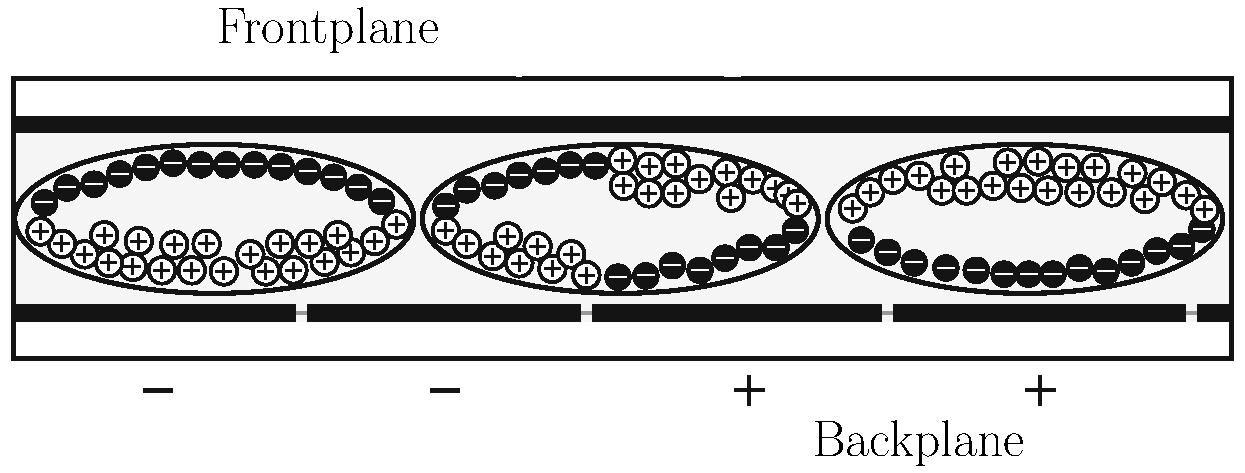
\includegraphics[width=0.9\textwidth]{2-theory/e-paper-display/graphics/capsules.pdf}
	\caption{Capsules between to electrodes (taken from \cite{amundson} with adjustments).\label{theory:capsules}}
\end{figure}

Each capsule in the film itself contains a transparent fluid and particles of two opposite charges.
One type of particle scatters the light while the other one absorbs it.
The particles now begin to move in opposite directions through the fluid when exposed two an electrical field. 
The pixel (defined by the electrode size) appears white if the scattering particles are near the frontplane and black if otherwise.
If no voltage is applied to the electrodes, the particles maintain their last position.
This makes it possible, to switch off the power supply when no image update is needed. 
This is the reason why the power consumption can be strongly reduced compared to other types of display \cite{amundson}.

\begin{figure}[ht]
	\centering
	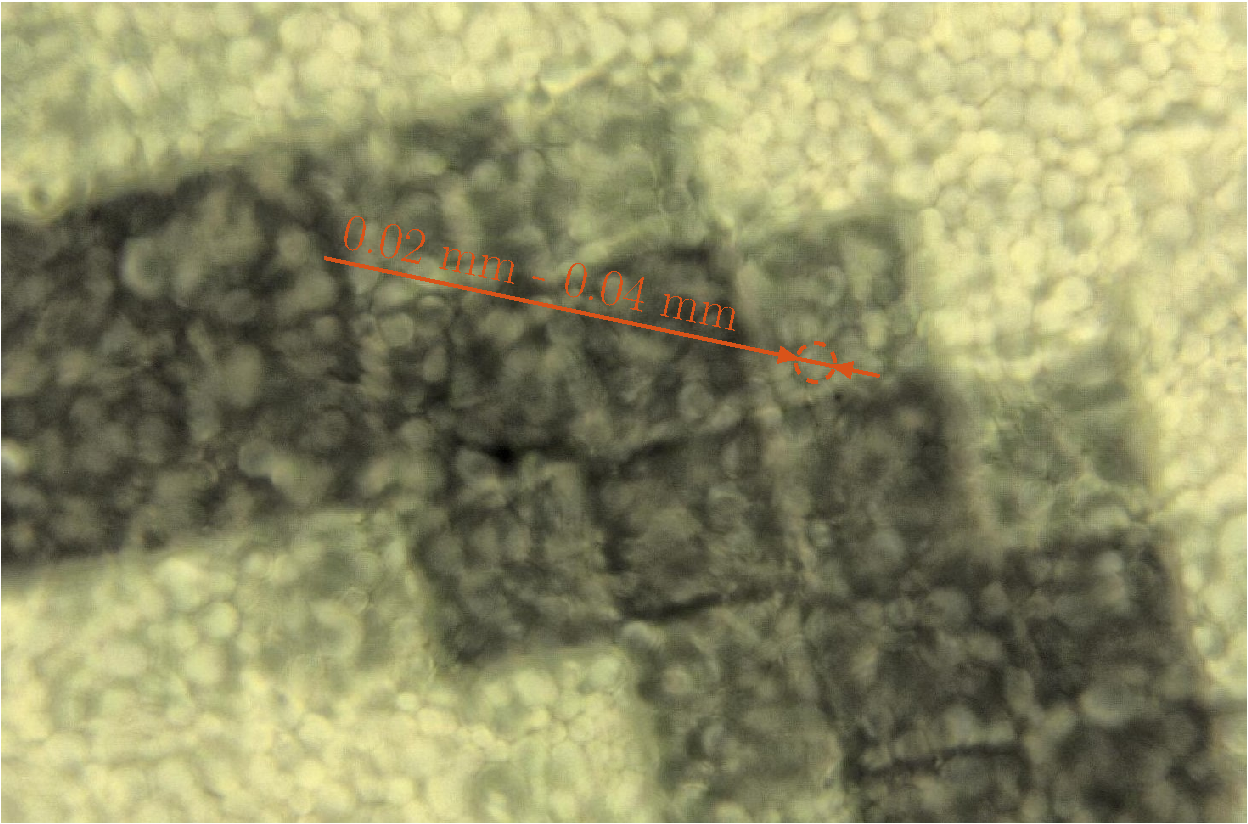
\includegraphics[width=0.9\textwidth]{2-theory/e-paper-display/graphics/epaper_mikroskop.pdf}
	\caption{E-paper display under microscope with 250x magnification.\label{theory:micro}}
\end{figure}

Figure \ref{theory:micro} shows an e-paper display with 250x magnification.